\documentclass{scrreprt}

\usepackage{amsmath,amssymb}
\usepackage{accsupp}
\usepackage[only,llbracket,rrbracket]{stmaryrd}
\usepackage[ntheorem]{empheq}
\usepackage{hyperref}
\usepackage{algorithm}
\usepackage{algpseudocode}
\usepackage{./shortcuts}

\usepackage{tikz}
\usetikzlibrary{backgrounds}

% sudo apt-get install pgf
\usepackage{pgfplots}
\pgfplotsset{compat=newest}

\begin{document}
\title{Using Peano's space-tree traversal for explicit
discontinuous Galerkin methods}
\author{Dominic Etienne Charrier}
\date{\today}
\maketitle
%%%%%%%%%%%%%%%%%%%%%%%%%%%%%%%%%%%%%%%%%%%%%%%%%%%%%%%%%%%
%%%%%%%%%%%%%%%%%%%%%%%%%%%%%%%%%%%%%%%%%%%%%%%%%%%%%%%%%%%
\chapter{Introduction}
%%%%%%%%%%%%%%%%%%%%%%%%%%%%%%%%%%%%%%%%%%%%%%%%%%%%%%%%%%%
%%%%%%%%%%%%%%%%%%%%%%%%%%%%%%%%%%%%%%%%%%%%%%%%%%%%%%%%%%%
We show how to use Peano's core functionality, the space-tree traversal,
and Peano's patch toolbox to solve partial differential
equations of the evolution type (parabolic, hyperbolic) using
explicit discontinuous Galerkin (DG) methods.

To this end, we discuss a linear advection problem.
The governing equations are discretized according
the method of lines. For the discretization in time, we employ an explicit
Euler time marching scheme.
We discretize the governing equations in space using an upwind DG formulation.
While this is a rather simple setup, it already covers most of the
steps that have to be performed for a wide range of linear
hyperbolic problems and their corresponding explicit DG discretizations.
%%%%%%%%%%%%%%%%%%%%%%%%%%%%%%%%%%%%%%%%%%%%%%%%%%%%%%%%%%%
%%%%%%%%%%%%%%%%%%%%%%%%%%%%%%%%%%%%%%%%%%%%%%%%%%%%%%%%%%%
\section{Preliminaries}
%%%%%%%%%%%%%%%%%%%%%%%%%%%%%%%%%%%%%%%%%%%%%%%%%%%%%%%%%%%
%%%%%%%%%%%%%%%%%%%%%%%%%%%%%%%%%%%%%%%%%%%%%%%%%%%%%%%%%%%
The (classical) divergence $\boldsymbol{\nabla}\cdot\vec{T}$ (a vector-valued
function) of a sufficiently regular second-order tensor-valued function
$\vec{T}$ is defined according to:
\begin{align}
(\boldsymbol{\nabla}\cdot\vec{T})_{i} &= \sum_{j=1}^d
\frac{\partial}{\partial x_j} T_{ij},\qquad
i=1,\ldots,N_{\textup{var}}
\end{align}
where $N_\textup{var}$ denotes the number of variables
and $d$ the space dimension.

% Furthermore, the (classical) tensor-valued gradient
% $\boldsymbol{\nabla}\vec{v}$ of a vector-valued function $\vec{v}$
% is defined by:}
% (\boldsymbol{\nabla}\vec{v})_{ij}
% &=
% \frac{\partial}{\partial x_j} v_i,\qquad
% i=1,\ldots,N_{\textup{var}},\;
% j=1,\ldots,d,
% Lastly, the scalar-valued double-dot product of two
% $\boldsymbol{\nabla}\vec{v}$ of a vector-valued function $\vec{v}$
% is defined by: }
%
% \end{align}

%%%%%%%%%%%%%%%%%%%%%%%%%%%%%%%%%%%%%%%%%%%%%%%%%%%%%%%%%%%
%%%%%%%%%%%%%%%%%%%%%%%%%%%%%%%%%%%%%%%%%%%%%%%%%%%%%%%%%%%
\section{Governing equation}
%%%%%%%%%%%%%%%%%%%%%%%%%%%%%%%%%%%%%%%%%%%%%%%%%%%%%%%%%%%
%%%%%%%%%%%%%%%%%%%%%%%%%%%%%%%%%%%%%%%%%%%%%%%%%%%%%%%%%%%
Let $\domain \subset \mathbb{R}^d$, $d=2,3$, denote a rectangular domain
with boundary $\boundary$.
We want to model the time evolution of a material concentration
$u$ inside of a flow field $\vec{b}$ by means of the following
conservation law:
\begin{subequations}
\begin{align}
\label{eq:governing_equations:advection}
\frac{\partial u}{\partial t} + \boldsymbol{\nabla} \cdot\vec{F}(u) &= 0&&
\textup{in } \domain \times (0,T],
\\
u(\xvec,0) &= u^0(\xvec)&& \textup{in }
\domain \times \{0\},
\end{align}
with $u^0$ denoting a sufficiently regular initial condition,
$T$ denoting the simulation time, and
\begin{align}
\vec{F}(u) = \vec{b}\,u \in \mathbb{R}^{N_\textup{var}\times d}
\end{align}
denoting the second-order tensor-valued physical flux ($N_\textup{var}=1$).
Please note that $\vec{F}(u)$ and $\vec{b}$ are here defined as row vectors.
Here and below, $\vec{b}$ is assumed to be sufficiently regular.
To complete the problem formulation, the material concentration is
further subject to sufficiently regular inflow boundary conditions, i.e.,
\begin{align}
\label{eq:governing_equations:advection_inflow}
u(\xvec,t) &= \inflow (\xvec,t),&& (\xvec,t) \in \boundaryIn
\times (0,T].
\end{align}
\end{subequations}
%%%%%%%%%%%%%%%%%%%%%%%%%%%%%%%%%%%%%%%%%%%%%%%%%%%%%%%%%%%
%%%%%%%%%%%%%%%%%%%%%%%%%%%%%%%%%%%%%%%%%%%%%%%%%%%%%%%%%%%
\chapter{An explicit one-step discontinuous Galerkin method
for linear advection}
\section{Computational mesh and trace operators}
\label{sec:mesh}
%%%%%%%%%%%%%%%%%%%%%%%%%%%%%%%%%%%%%%%%%%%%%%%%%%%%%%%%%%%
%%%%%%%%%%%%%%%%%%%%%%%%%%%%%%%%%%%%%%%%%%%%%%%%%%%%%%%%%%%
Let $\tria$ be a structured Cartesian mesh on $\domain\subset\mathbb{R}$.
We refer to the disjoint open sets $\cell \in \tria$ as elements. We denote by $\hcell$
the diameter of $\cell$.
We store the local quantities $\hcell$ in the vector
$\laVec{h} = \{ \hcell \}_{\cell \in \tria}$, and
set
$h_\textup{max} = \text{max}_{\cell \in \tria }\,\hcell$.
Finally, $\normal$ denotes the outward normal unit vector to the element boundary
$\cellBnd$. We will denote the number of elements by $\Ncell$.

An interior face of $\tria$ is the $d-1$ dimensional intersection
$\cellBnd^{+} \cap \cellBnd^{-}$, where $\cellPlus$ and $\cellMinus$
are two adjacent elements of $\tria$. Similarly, a boundary face of $\tria$ is
the $d-1$ dimensional intersection $\cellBnd \cap \boundary$ which consists
of entire faces of $\cellBnd$.
We denote by $\internalFaces$ the union of all interior faces of $\tria$.

Here and in the following, we refer generically to a ``face" even in the
case $d=2$.
Now, let $\face \in \internalFaces$ be an interior face shared by
the elements $\cellPlus$ and $\cellMinus$.
We denote by $\varphi$ a scalar-valued function (in
$\sobolev{1}{\tria}$).
We observe that the traces of $\varphi$
are defined twice on $\face$.
Let $\varphi^{\pm}$ denote the trace of $\varphi$ on $\face$ from the
interior of $\cell^{\pm}$;
we define a jump operator $\jmp{\varphi\normal}$ by
\begin{align}
\jmp{\varphi\normal} &= \varphi^{+}\normal^{+} + \varphi^{-}\normal^{-}.
\end{align}
%%%%%%%%%%%%%%%%%%%%%%%%%%%%%%%%%%%%%%%%%%%%%%%%%%%%%%%%%%%
%%%%%%%%%%%%%%%%%%%%%%%%%%%%%%%%%%%%%%%%%%%%%%%%%%%%%%%%%%%
\section{Discretization of the linear advection problem}
%%%%%%%%%%%%%%%%%%%%%%%%%%%%%%%%%%%%%%%%%%%%%%%%%%%%%%%%%%%
%%%%%%%%%%%%%%%%%%%%%%%%%%%%%%%%%%%%%%%%%%%%%%%%%%%%%%%%%%%
We discretize \eqref{eq:governing_equations:advection} -- \eqref{eq:governing_equations:advection_inflow}
following the method of lines procedure. Thus, we make the ansatz
\begin{align}
u_h (\xvec,t) = \sum_m u_m (t)\,\phi_i(\vec{x}),
\end{align}
with time-dependent coefficients $u_i$, and basis
functions $\vec{\phi}_i$ that depend solely on $\vec{x}$ and belong
to the discrete space
\begin{align}
\mathcal{V}_h &= \left \{
v_h \in \lebesgueTwo{\Omega}: v_h|_\cell \in
{Q}_N(\cell),\, \forall \cell \in \tria
\right \}
\end{align}
with $N$ denoting the order of approximation, and
${Q}_N(\cell)$ denoting the space of polynomials of
degree at most $N$.
Note that the above ansatz uses indices in terms of a global basis.
It is however often more useful to introduce a local
basis function index. This index together with the index of the element the basis function
``lives in'' can then be mapped to a global index if necessary.
Thus, we make the following ansatz instead:
\begin{align}
u_h (\xvec,t) =
\sum_{c=1}^{\Ncell}\,\sum_{i=1}^{N_{\textup{basis}}} u_{c,m}
(t)\,\phi_{c,m}(\vec{x}),
\end{align}

Furthermore, for any boundary face $\face\in\boundaryOut$
of the mesh, we introduce inflow (``$\downarrow$'') and outflow
(``$\uparrow$'') parts
\begin{align}
\face^{\downarrow} &= \{ \vec{x} \in \face :(\vec{b} \cdot
\normal)(\vec{x}) < 0\},\qquad
\face^{\uparrow} = \{ \vec{x} \in \face : (\vec{b} \cdot\normal)(\vec{x})
\geq 0\}.
\end{align}
With respect to the previous definitions, the semidiscrete upwind DG
formulation of problem \eqref{eq:governing_equations:advection} -- \eqref{eq:governing_equations:advection_inflow}
consists of
finding a sufficient regular $u_h\in\mathcal{V}_h$ such that
\begin{align}
\sumCells \intCell \frac{\partial}{\partial t}u_h\,v_h\,\dV
&=
\sumCells \intCell \vec{F}(u_h) \cdot \nabla v_h\,\dV
- \sum_{\face \in \internalFaces} \int_\face
\vec{G}(u_h^{+},u_h^{-})\cdot\jmp{v_h \normal}\,\ds
\\
&- \sum_{\face \in \boundary} \int_{\face^{\uparrow}}
\vec{F}(u_h) \cdot \normal \,v_h\,\ds
- \sum_{\face \in \boundary} \int_{\face^{\downarrow}}
(\vec{F}(\inflow)\cdot\normal)\,v_h\,\ds,
\qquad\forall v_h \in\mathcal{V}_h.
\notag
\end{align}
The above equations are the result of elementwise partial integration
and a consequent summation over all elements.
To complete the DG formulation, we have to define unique values
on the interior faces, the so-called numerical fluxes here denoted by
$\vec{G}^{*}(u_h^{+},u_h^{-})$.
Above, we have decided to use so-called upwind fluxes, i.e.,
we choose,
\begin{align}
\vec{G}(u_h^{+},u_h^{-}) = u_h^{\uparrow}\,\vec{b}.
\end{align}
where we have defined the upstream/upwind value (``$\uparrow$'')
of $u_h$ according to
\begin{align}
u_h^{\uparrow}(\xvec) &=
\begin{cases}
u_h^{+}&(\vec{b} \cdot \normal^{+})(\vec{x}) \geq 0,
\\
u_h^{-}&(\vec{b} \cdot \normal^{-})(\vec{x}) > 0,
\end{cases}
\end{align}
with $\vec{x} \in \face$ and $u_h^{\pm}=u_h|_{\cell^{\pm}}$.

Note that the choice of the fluxes has effects on both,
the stability and the order of convergence of a DG method
Note further that for the linear advection equation,
many numerical fluxes, e.g., Lax-Friedrichs, HLLE, etc., reduce to the above
upwind flux. One particluar exception is the central flux which leads to an
unstable method; cf.~\cite{hartmann_2008} for a source of all of the statements
above.

After the choice of the fluxes, we need to choose a basis
of the space $\mathcal{V}_h$ to complete the spatial discretization.
We give examples for such a basis in the next sections.

If we choose a basis, the above discrete variational problem is equivalent
to the following system of ordinary differential equations:
\begin{align}
\label{eq:advection:ode_system}
\laMat{M}\,\frac{\text{d}}{\text{d}t}\laVec{u}(t)
&= (\laMat{F}\,
+ \laMat{G}
+ \laMat{O})\,\laVec{u}(t)
+ \laVec{I}(t)
,&&\textup{almost everywhere in } (0,T),
\intertext{s.t. the initial conditions}
\laVec{u}(0) &= \laVec{u}^0,
\end{align}
with the vector $\laVec{u}(t)$ containing the time-dependent coefficients
to the time-independent basis functions.
Note that only the operation $\laMat{G}\,\laVec{u}$ is non-local
and requires communication between processes.
Note further that the mass operator $\laMat{M}$ is in general
block-diagonal or even diagonal if an $L^2(\domain)$-orthogonal basis is used.
We will further refer to $\laMat{F}$ as the volume flux operator, to
$\laMat{O}$ as the outflow operator,
to $\laMat{G}$ as the normal flux operator,
and to $\laMat{I}$ as the inflow vector.
We will clarify in the next sections which bilinear forms appearing
in the above variational problem are mapped to which operator.
Note that we use the term operator since our implementation is
matrix-free, i.e., we will not assemble any global matrices.

We discretize \ref{eq:advection:ode_system} in time using an explicit (one-step)
forward Euler method. This results in the update scheme below:
\begin{align}
\laVec{u}^{l+1}
&=
\laVec{u}^{l}
+
\Delta t\,\laMat{M}^{-1}\left((\laMat{F}\,
+ \laMat{O})\,\laVec{u}^l
+ \laVec{I}(t^l)
+ \laMat{G}\,\laVec{u}^{l}
\right),
\end{align}
with $l=0,\ldots,l_{max}$ denoting the time step, $t^l$ denoting a discrete
point in time, and $\Delta t$ denoting the time step size. The maximum time step depends
on the simulation time according to $l_{max}=T/\Delta t$.

To ensure stability of the scheme, we have to limit the size of time step.
For global time stepping schemes as ours, the upper bound for admissible time
steps is usually estimated according to:
\begin{align}
\label{eq:cfl_time_step}
\Delta
t <
\textup{CFL}\,\max_{\cell\in\tria}\,\left\{
\frac{\varrho_\cell}{\max_{\xvec\in\cell}|\vec{b}|}
\right\},
\end{align}
with $\textup{CFL}=(2\,N+1)^{-1}$ (cf.~e.g.~\cite{cockburn_book}), where $N$
denotes the polynomial order of the spatial discretization.
Here, $\rho_K$ denotes the smallest circle that can be inscribed inside
the grid cell $\cell$.
\begin{remark}
{\rm
For cellwise constant DG methods on Cartesian grids, the CFL condition can be
interpreted the following way:
}
During a time step,
information is only allowed to flow to the direct neighbors of
a cell.
\end{remark}
\begin{remark}
{\rm
Note that the CFL criterion imposes a severe restriction on the
time step size if we want to use higher order spatial approximations
($N>0$).}
\end{remark}
%%%%%%%%%%%%%%%%%%%%%%%%%%%%%%%%%%%%%%%%%%%%%%%%%%%%%%%%%%%
%%%%%%%%%%%%%%%%%%%%%%%%%%%%%%%%%%%%%%%%%%%%%%%%%%%%%%%%%%%
\section{The local discrete operators}
%%%%%%%%%%%%%%%%%%%%%%%%%%%%%%%%%%%%%%%%%%%%%%%%%%%%%%%%%%%
%%%%%%%%%%%%%%%%%%%%%%%%%%%%%%%%%%%%%%%%%%%%%%%%%%%%%%%%%%%
\subsection{Preliminaries}
We store all cells of the mesh in an ordered list $\{
\cell_c \}_{1 \leq c \leq \Ncell}$.

Recall that we construct a global basis
for $\mathcal{V}_h$ using local basis
functions with compact support on each cell $\cell_c$, i.e., the basis functions
attain non-zero values only in one particular cell $\cell_c$ and are identical
to zero elsewhere.

We denote by $\{ \phiCell{c}{m} \}_{1 \leq m \leq
\NphiCell}$ the local basis in $\cell_c$,
with $\NphiCell$ denoting the size of the local basis.
Note that for an approximation of order N, the size of the local basis is
computed according to:
\begin{align}
\NphiCell = 1\times(N+1)^d.
\end{align}
There are many different ways to choose the basis functions.
Usual choices are nodal basis functions (Lagrange polynomials) or
modal basis functions (Legendre polynomials).
The latter and certain nodal basis functions where the nodes are located at
Gauss-Legendre quadrature points have a useful property:
They are orthogonal in the $L^2(\Omega)$ sense.
Choosing such a basis often results in very sparse operators, e.g.,
the mass operator is completely diagonal in this case.

We will further define $u_h^c=u_h|_{\cell_c}$.
To derive the elements of the operators introduced
in the previous section, we can apply the following replacement rule:
\begin{align}
u_h^{c} &\rightarrow \phiCell{c}{n} & \textup{specifies a column}, \\
v_h^{c} &\rightarrow \phiCell{c}{m} & \textup{specifies a row},
\end{align}
where $u_h\in\mathcal{V}_h$ refers to the ansatz function and
$v_h\in\mathcal{V}_h$ to a test function.
Lastly, if two cells share a face, we will always indicate the
neighbor cell by the index $b$, and the ``current''cell
by the index $c$.
%%%%%%%%%%%%%%%%%%%%%%%%%%%%%%%%%%%%%%%%%%%%%%%%%%%%%%%%%%%
\subsection{Mass operator}
%%%%%%%%%%%%%%%%%%%%%%%%%%%%%%%%%%%%%%%%%%%%%%%%%%%%%%%%%%%
Thanks to the compact support of the local basis functions,
we only have to compute the local block matrix
$\laMat{M}^{c,c} \in \mathbb{R}^{\NphiCell \times \NphiCell}$ for each
cell $\cell_c$, where
\begin{align}
\mathrm{M}^{c,c}_{m,n} =
\int_{\cell_c}
\phiCell{c}{m}\,\phiCell{c}{n} \, \dV,
&& m,n = 1,\ldots,\NphiCell.
\end{align}
The mass operator is thus in general block-diagonal.
\subsection{Volume flux operator}
Thanks to the compact support of the local basis functions,
we only have to compute the local block matrix
$\laMat{F}^{c,c} \in \mathbb{R}^{\NphiCell \times \NphiCell}$ for each
cell $\cell_c$, where
\begin{align}
\label{eq:volume_flux_op}
\mathrm{F}^{c,c}_{m,n} &= \sumCells \intCell \vec{F}(\phiCell{c}{n}) \cdot
\nabla \phiCell{c}{m}\,\dV
&& m,n = 1,\ldots,\NphiCell.
\end{align}
The volume flux operator is thus in general block-diagonal.
\subsection{Outflow operator}
Let us denote the outflow part of a face from the perspective of cell $\cell_c$
by
\begin{align}
\face^{c,\uparrow} \isdef \{ \vec{x} \in \face : (\vec{b} \cdot
\cellNormal{c})(\vec{x})> 0\}.
\end{align}
Let $\face \subset \boundary \cap \cellBnd_c$, where $\cellBnd_c$
denotes the boundary of cell $\cell_c$.
Thanks to the compact support of the local basis functions, we only
have to compute the local matrix $\laMat{O}^{c,c} \in \mathbb{R}^{\NphiCell
\times \NphiCell}$ for each cell $\cell_c$, where
\begin{align}
\mathrm{O}^{c,c}_{m,n} =
\int_{\face^{c,\uparrow}}
-
(\vec{F}(\phiCell{c}{n})\cdot\normal)\,\phiCell{c}{m} \, \dV,
&& m,n = 1,\ldots,\NphiCell.
\end{align}
The outflow operator is thus in general block-diagonal.
\subsection{Inflow vector}
Let us denote the inflow part of a face from the perspective of cell $\cell_c$
by
\begin{align}
\face^{c,\downarrow} \isdef \{ \vec{x} \in \face : (\vec{b} \cdot
\cellNormal{c})(\vec{x}) < 0\}
\end{align}
Thanks to the compact support of the local basis functions, we only
have to compute the local vector $\laMat{I}^{c} \in \mathbb{R}^{\NphiCell
\times \NphiCell}$ for each cell $\cell_c$, where
\begin{align}
\mathrm{I}^{c}_{m} =
\int_{\face^{c,\downarrow}}
j(t^n)\,\phiCell{c}{m} \, \dV,
&& m,n = 1,\ldots,\NphiCell.
\end{align}
\begin{remark}
Compact support
\rm {should sound familiar at this point.}
\end{remark}
\section{The non-local discrete normal flux operator}
Let the face $\face \in \internalFaces$ be part of the boundary of both
cells $\cell_c$ and $\cell_b$, we have to compute the block matrices
$\laMat{G}_\face^{c,c} \in \mathbb{R}^{\NphiCell \times \NphiCell}$,
$\laMat{G}^{c,b} \in \mathbb{R}^{\NphiCell \times \NphiCell}$,
$\laMat{G}^{b,c} \in \mathbb{R}^{\NphiCell \times \NphiCell}$,
and
$\laMat{G}^{b,b} \in \mathbb{R}^{\NphiCell \times \NphiCell}$
according to:
\begin{align}
{G}^{c,c}_{\face;m,n} &=
\int_{\face}
-
\vec{G}^{\uparrow}(\phiCell{c}{n},\cellNormal{c})\cdot\cellNormal{c}\,
\phiCell{c}{m} \, \dV,
&& m,n = 1,\ldots,\NphiCell,
\\
{G}^{c,b}_{m,n} &=
\int_{\face}
\vec{G}^{\uparrow}(\phiCell{b}{n},\cellNormal{b})\cdot\cellNormal{b}\,
\phiCell{c}{m} \, \dV,
&& m,n = 1,\ldots,\NphiCell,
\\
\intertext{and}
\\
{G}^{b,b}_{\face;m,n} &=
\int_{\face}
-
\vec{G}^{\uparrow}(\phiCell{b}{n},\cellNormal{b})
\cdot \cellNormal{b}
\,
\phiCell{b}{m} \, \dV,
&& m,n = 1,\ldots,\NphiCell,
\\
{G}^{b,c}_{m,n} &=
\int_{\face}
\vec{G}^{\uparrow}(\phiCell{c}{n},\cellNormal{c})
\cdot \cellNormal{c}
\,\phiCell{b}{m} \, \dV,
&& m,n = 1,\ldots,\NphiCell.
\end{align}
Above, we have introduced
\begin{align}
\vec{G}^{\uparrow}(\phiCell{+}{n},\normal)
&=
\begin{cases}
\vec{b}\,\phiCell{+}{n}
& \textup{for }
(\vec{b} \cdot \normal)(\vec{x}) \geq 0,
\\
0                & \textup{otherwise},
\end{cases}
\end{align}
Note that we write once per face, i.e., maximum  $2\,d$ times, to the block
$\laMat{G}^{c,c}$:
\begin{align}
\laMat{G}^{c,c} &= \sum_{\substack{\face\subset\cellBnd \\
\face\in\internalFaces}}\laMat{G}^{c,c}_{\face} =
\sum_{i=1}^{2\,d}\laMat{G}^{c,c}_{\face_i}.
\end{align}
On Cartesian grids, we can combine the contributions made by pairs of opposite
neighbors of the current cell $\cell_c$ by defining so-called fluctuations.
Let us indicate the left, right, front, and back neighbor of cell $\cell_c$ by
$\textup{left}(c)$, $\textup{right}(c)$, $\textup{front}(c)$,
and $\textup{back}(c)$, respectively
If we write the neighbor contributions
down in terms of fluctuations, we obtain:
\begin{align}
\mathrm{D}^c_{x;m} (u_{n}^{\textup{left}(c)},u_{n}^{\textup{right}(c)}) &=
\mathrm{G}_{m,n}^{c,\textup{right}(c)}\,u_{n}^{\textup{right}(c)} +
\mathrm{G}_{m,n}^{c,\textup{left}(c)}\,u_{n}^{\textup{left}(c)} \\
&=
\left(-\int_{\face}
\vec{G}^{\uparrow}(\phiCell{\textup{right}(c)}{n},-\normal_x)
\cdot\normal_x\,
\phiCell{c}{m} \, \dV\right)
\,u_{n}^{\textup{right}(c)} 
\\
&-
\left(-\int_{\face}
\vec{G}^{\uparrow}(\phiCell{\textup{left}(c)}{n},\normal_x)
\cdot\normal_x\,
\phiCell{c}{m} \, \dV\right)
\,u_{n}^{\textup{left}(c)},
\\
\mathrm{D}^c_{y;m} (u_{n}^{\textup{front}(c)},u_{n}^{\textup{back}(c)}) &= 
\mathrm{G}_{m,n}^{c,\textup{back}(c)}\,u_{n}^{\textup{back}(c)}
+ \mathrm{G}_{m,n}^{c,\textup{front}(c)}\,u_{n}^{\textup{front}(c)} \\
&=
\left(-\int_{\face}
\vec{G}^{\uparrow}(\phiCell{\textup{back}(c)}{n},-\normal_y)
\cdot\normal_y\,
\phiCell{c}{m} \, \dV\right)
\,u_{n}^{\textup{back}(c)} 
\\
&-
\left(-\int_{\face}
\vec{G}^{\uparrow}(\phiCell{\textup{front}(c)}{n},\normal_y)
\cdot\normal_y\,
\phiCell{c}{m} \, \dV\right)
\,u_{n}^{\textup{front}(c)},
\end{align}
with $\normal_x=(1,0)^\textup{T}$, and $\normal_y=(0,1)^\textup{T}$.
%%%%%%%%%%%%%%%%%%%%%%%%%%%%%%%%%%%%%%%%%%%%%%%%%%%%%%%%%%%
%%%%%%%%%%%%%%%%%%%%%%%%%%%%%%%%%%%%%%%%%%%%%%%%%%%%%%%%%%%
\section{Cellwise constant basis functions (in space)}
%%%%%%%%%%%%%%%%%%%%%%%%%%%%%%%%%%%%%%%%%%%%%%%%%%%%%%%%%%%
%%%%%%%%%%%%%%%%%%%%%%%%%%%%%%%%%%%%%%%%%%%%%%%%%%%%%%%%%%%
In the case of cellwise constant basis functions, we can make the following
simplifications. Let $\cell_c\in\tria$; the mass operator
is diagonal and has one element per cell:
\begin{align}
\mathrm{M}^{c,c} =
\int_{\cell_c} 1\,\dV = | \cell_c |
&\Leftrightarrow (\mathrm{M}^{-1})^{c,c} =
1/| \cell_c |,
\intertext{The volume fluxes are identical to zero, i.e.,}
\laMat{F} &= 0,
\intertext{since the gradient of the cellwise constant basis functions is
identical to zero.
The outflow operator is diagonal and has one element per cell:}
\mathrm{O}^{c,c} =
\int_{\face^{c,+}}
\vec{F}(1)\cdot\normal\,\, \dV
&=
\int_{\face^{c,+}}
\vec{b}\cdot\normal\,\, \dV,
\intertext{and the inflow vector has one element in each cell:}
\mathrm{I}^{c} &=
\int_{\face^{c,\downarrow}}
j(t^n) \, \dV,
\end{align}
\begin{align}
\intertext{We have the following contributions to the normal flux
operator per face:}
\mathrm{G}_\face^{c,c} &=
\int_{\face}
-
\vec{G}^{\uparrow}(1,\cellNormal{c})\,\cellNormal{c}\,\dV,
\\
\mathrm{G}^{c,b} &=
\int_{\face}
\vec{G}^{\uparrow}(1,\cellNormal{b})\,\cellNormal{b}\, \dV,
\\
\intertext{and}
\\
\mathrm{G}_\face^{b,b} &=
\int_{\face}
-
\vec{G}^{\uparrow}(1,\cellNormal{b})\,\cellNormal{b}\, \dV,
\\
\mathrm{G}^{b,c} &=
\int_{\face}
\vec{G}^{\uparrow}(1,\cellNormal{c})\,\cellNormal{c}\,\dV.
\end{align}
The fluctuations simplify to
\begin{align}
\mathrm{D}^c_{x} (u^{\textup{left}(c)},u^{\textup{right}(c)}) &=
\mathrm{G}^{c,\textup{right}(c)}\,u^{\textup{right}(c)} +
\mathrm{G}^{c,\textup{left}(c)}\,u^{\textup{left}(c)} \\
&=
\left(-\int_{\face}
\vec{G}^{\uparrow}(1,-\normal_x)
\cdot\normal_x\,\dV\right)
\,u^{\textup{right}(c)} 
\\
&-
\left(-\int_{\face}
\vec{G}^{\uparrow}(1,\normal_x)
\cdot\normal_x\, \dV\right)
\,u^{\textup{left}(c)},
\\
\mathrm{D}^c_{y} (u^{\textup{front}(c)},u^{\textup{back}(c)}) &= 
\mathrm{G}^{c,\textup{back}(c)}\,u^{\textup{back}(c)}
+ \mathrm{G}^{c,\textup{front}(c)}\,u^{\textup{front}(c)} \\
&=
\left(-\int_{\face}
\vec{G}^{\uparrow}(1,-\normal_y)
\cdot\normal_y\, \dV\right)
\,u_{n}^{\textup{back}(c)} 
\\
&-
\left(-\int_{\face}
\vec{G}^{\uparrow}(1,\normal_y)
\cdot\normal_y\, \dV\right)
\,u_{n}^{\textup{front}(c)},
\end{align}
\subsection{Cell updates}
In each time step, we thus update the cell according to:
\begin{align}
u^{c;n+1} &= u^{c;n} + \Delta u^{c;n}
\intertext{with}
\Delta u^{c;n} &= \Delta t\,|\cell|^{-1} \left( \mathrm{O^{c,c}}u^{c;n} +
\sum_{i=1}^{2\,d}\mathrm{G}^{c,c}_{\face_i}u^{c;n} \right)\\
&+
 \Delta t\,|\cell|^{-1}\,\mathrm{D}^c_{x}
 (u^{\textup{left}(c);n},u^{\textup{right}(c);n}) \\
 &+
 \Delta t\,|\cell|^{-1}\,
 \mathrm{D}^c_{y} (u^{\textup{front}(c);n},u^{\textup{back}(c);n}).
\end{align}
\subsection{Cell updates}
%%%%%%%%%%%%%%%%%%%%%%%%%%%%%%%%%%%%%%%%%%%%%%%%%%%%%%%%%%%
%%%%%%%%%%%%%%%%%%%%%%%%%%%%%%%%%%%%%%%%%%%%%%%%%%%%%%%%%%%
\section{Mappings}
%%%%%%%%%%%%%%%%%%%%%%%%%%%%%%%%%%%%%%%%%%%%%%%%%%%%%%%%%%%
%%%%%%%%%%%%%%%%%%%%%%%%%%%%%%%%%%%%%%%%%%%%%%%%%%%%%%%%%%%
In this section, we introduce mappings between the mesh elements
$\cell\in\tria$ and a reference element. These mappings allow
us to treat integrals over arbitrarily shaped mesh elements in an uniform manner.
To ease the presentation, we only consider the two-dimensional case.
\\[5pt]
Let us define the \textit{reference element} ${\refCell=[-1,1]^2}$
and let us denote by $\refVec{x}=(\hat{x},\hat{y})\transp$ a point belonging to $\refCell$.
Let $\cell\in\tria$ denote a quadrilateral element
and let its corners $\vec{P}_m$, $m=1,2,3,4$, be ordered as shown in figure \ref{fig:stokes_ipdg_impl:node_ordering}.
\begin{figure}[h]
\centering
\tikzset{dot/.style={circle,fill=#1,inner sep=0,minimum size=4pt}}
\begin{tikzpicture}
%
\path[draw] (-1,-1) -- (1,-1) -- (1,1) -- (-1,1) -- (-1,-1);
%
\node [circle=green,fill=white,scale=0.8] at (-1,-1) {\textbf{1}};
\node [circle=green,fill=white,scale=0.8] at ( 1,-1) {\textbf{2}};
\node [circle=green,fill=white,scale=0.8] at (-1, 1) {\textbf{3}};
\node [circle=green,fill=white,scale=0.8] at ( 1, 1) {\textbf{4}};
\end{tikzpicture}
\caption[Node ordering]{Node ordering}
\label{fig:stokes_ipdg_impl:node_ordering}
\end{figure}
\\
For simplicity, we assume that the quadrilateral $\cell$ has straight edges.
Then, we can express $\cell$ according to
\begin{align}
\cell &= \mapping (\refCell),
\notag
\intertext{where we define the mapping $\mapping : \refCell \to \cell$ by}
\label{eq:stokes_ipdg_impl:mapping}
\vec{x} = \mapping(\refVec{x})
&=
\begin{pmatrix}
\mappingT{x}(\refVec{x})\\
\mappingT{y}(\refVec{x})
\end{pmatrix}
= \sum_{m=1}^4 \vec{P}_{m}\,s_m(\refVec{x}),
\qquad \refVec{x}\in\refCell,\vec{x}\in\cell.
\end{align}
The \textit{shape functions} $s_m(\refVec{x})$, $m=1,2,3,4$, are defined according to
\begin{align}
\label{eq:stokes_ipdg_impl:shape_fun_1}
s_1(\refVec{x})
&=
\frac{1}{4}(1-\hat{x})\,(1-\hat{y}),
\qquad
s_3(\refVec{x})
=
\frac{1}{4}(1-\hat{x})\,(1+\hat{y}),
\\
\label{eq:stokes_ipdg_impl:shape_fun_4}
s_2(\refVec{x})
&=
\frac{1}{4}(1+\hat{x})\,(1-\hat{y}),
\qquad
s_4(\refVec{x})
=
\frac{1}{4}(1+\hat{x})\,(1+\hat{y}),
\intertext{and have the property}
s_m(\refVec{P}_n) &=
\begin{cases}
1,&m=n,\\
0,&m\neq n,
\end{cases}
\end{align}
where $\refVec{P}_1=(-1,-1)\transp$, $\refVec{P}_2=(1,-1)\transp$, $\refVec{P}_3=(-1,1)\transp$, and $\refVec{P}_4=(1,1)\transp$ denote the
corner points of the reference element. Note that the indexing of these corner points is in compliance with the node ordering depicted in
figure \ref{fig:stokes_ipdg_impl:node_ordering}.

Note that in case of Cartesian elements, we can simplify the above
mapping according to:
\begin{align}
\vec{x} = \mapping(\refVec{x})
&=
\vec{P}_{\textup{center}} +
\frac{1}{2}
\begin{pmatrix}
\Delta x & 0 \\
0 & \Delta y
\end{pmatrix}
\begin{pmatrix}
\hat{x} \\
\hat{y}
\end{pmatrix},
\end{align}
where $\Delta x$ and $\Delta y$ denote the dimensions of the element in the
respective coordinate direction.
Note that $\vec{P}_{\textup{center}}$ is the center of the element.

Assuming it exists, we denote the inverse mapping by $\imapping : \cell \to \refCell$, which
in general cannot be constructed by polynomial shape functions.
Next, let us define the Jacobian matrix
\begin{align}
\jacobian (\refVec{x})&=
\begin{pmatrix}
\jacobianT{x}{\hat{x}} & \jacobianT{x}{\hat{y}} \\
\jacobianT{y}{\hat{x}} & \jacobianT{y}{\hat{y}}
\end{pmatrix}(\refVec{x}),
\notag
\intertext{and its determinant}
\detJ(\refVec{x}) = \textup{det}\left(\jacobian\right)(\refVec{x})&=
\begin{vmatrix}
\jacobianT{x}{\hat{x}} & \jacobianT{x}{\hat{y}} \\
\jacobianT{y}{\hat{x}} & \jacobianT{y}{\hat{y}}
\end{vmatrix}(\refVec{x}).
\notag
\end{align}
Assume that $\mapping$ is invertible, we accordingly define
$\ijacobian (\vec{x})$ and it follows from the inverse function theorem that
\begin{align}
\ijacobian (\vec{x}) &= \left(\jacobian\right)^{-1}(\refVec{x}),
\notag
\end{align}
for $\refVec{x}\in\refCell$ such that $\vec{x}=\mapping(\refVec{x})\in\cell$.
We note that if the element $\cell$ is affine,
it holds that
\begin{align}
\jacobian (\refVec{x}) = \jacobian = \textup{const.}\qquad
&\Leftrightarrow
\qquad\detJ (\refVec{x}) = \detJ = \textup{const.},
\notag
\intertext{and the mapping has the form}
\mapping(\refVec{x})
&=
\jacobian\cdot\refVec{x} + \vec{P}_1.
\notag
\end{align}
In this case, there exists an inverse mapping if
$\jacobian$ is regular, i.e. $\detJ\neq 0$.
\\[5pt]
According to an invertible mapping $\mapping$, we can further derive the following identity.
Let $\hat{f}$ be a sufficiently regular function on the reference element $\refCell$, and
let $f$ be sufficiently regular on $\cell$ and such that
\begin{align}
\label{eq:stokes_ipdg_impl:imapping_scalar_function}
f(\vec{x}) &= (\hat{f} \circ \imapping)(\vec{x}) = \hat{f}(\refVec{x}),
\qquad
\refVec{x}\in\refCell,\,\vec{x}=\mapping(\refVec{x})\in\cell.
\end{align}
Then, it holds that
\begin{align}
\nabla\,f(\vec{x}) &= \left(\jacobian^{-\textup{T}}\,\cdot\hat{\nabla}\,\hat{f}\right)(\refVec{x}),
\notag
\intertext{where}
\hat{\nabla} &= \left(\frac{\partialup}{\partialup \hat{x}},\,\frac{\partialup}{\partialup \hat{y}}\right)\transp
\notag
\end{align}
denotes the gradient with respect to the reference coordinates. This follows
from \eqref{eq:stokes_ipdg_impl:imapping_scalar_function} and using the chain rule.
A similar identity can be derived for vector-valued functions.
We can further express volume integrals over the element $\cell$
with respect to the reference coordinates and the invertible mapping $\mapping$.
Let $\hat{f}$ and $f$ be defined as in \eqref{eq:stokes_ipdg_impl:imapping_scalar_function},
we have
\begin{align}
\intCell f(\vec{x})\,\dV &= \intRefCell \hat{f}(\refVec{x})\,|\detJ(\refVec{x})|\,\refdV
=
\int_{-1}^1\int_{-1}^1 \hat{f}(\hat{x},\hat{y})\,|\detJ(\hat{x},\hat{y})|\,\refdV\,\refdy.
\notag
\end{align}
Further, if we define the faces of the reference element according to
\begin{align}
\refFace_{1} &= \{ \refVec{x} \in \refCell : \hat{x} = -1\},\qquad
\refFace_{3} = \{ \refVec{x} \in \refCell : \hat{y} = -1\},
\notag\\
\refFace_{2} &= \{ \refVec{x} \in \refCell : \hat{x} = +1\},\qquad
\refFace_{4} = \{ \refVec{x} \in \refCell : \hat{y} = +1\},
\notag
\end{align}
we can define the four faces belonging to the boundary of $\cell$ by
\begin{align}
\face_{1} &= \mapping(\refFace_1),\qquad
\face_{2} = \mapping(\refFace_2),\qquad
\face_{3} = \mapping(\refFace_3),\qquad
\face_{4} = \mapping(\refFace_4).
\notag
\end{align}
Now we can express integrals over faces belonging to the boundary of $\cell$ with respect to
the reference coordinates and the mapping $\mapping$.
Let $\hat{f}$ and $f$ be defined as in \eqref{eq:stokes_ipdg_impl:imapping_scalar_function},
we have
\begin{align}
\int_{\face_1} f(\vec{x})\,\ds &=
\int_{-1}^1\hat{f}(-1,\hat{y})\,\left|\frac{d\mapping(-1,\hat{y})}{\refdy}\right|\,\refdy,
\notag\\
\int_{\face_2} f(\vec{x})\,\ds &=
\int_{-1}^1\hat{f}(+1,\hat{y})\,\left|\frac{d\mapping(+1,\hat{y})}{\refdy}\right|\,\refdy,
\notag\\
\int_{\face_3} f(\vec{x})\,\ds &=
\int_{-1}^1\hat{f}(\hat{x},-1)\,\left|\frac{d\mapping(\hat{x},-1)}{\refdx}\right|\,\refdx,
\notag\\
\int_{\face_4} f(\vec{x})\,\ds &=
\int_{-1}^1\hat{f}(\hat{x},+1)\,\left|\frac{d\mapping(\hat{x},-1)}{\refdx}\right|\,\refdx.
\notag
\end{align}
Please note that all these concepts extend to the 3-d case and it is also
possible to use higher order shape functions instead of the linear
Lagrange polynomials that we used in \eqref{eq:stokes_ipdg_impl:shape_fun_1} and
\eqref{eq:stokes_ipdg_impl:shape_fun_4}; by linear we mean
linear in each reference coordinate direction.
%%%%%%%%%%%%%%%%%%%%%%%%%%%%%%%%%%%%%%%%%%%%%%%%%%%%%%%%%%%
%%%%%%%%%%%%%%%%%%%%%%%%%%%%%%%%%%%%%%%%%%%%%%%%%%%%%%%%%%%
\chapter{Implementation of the cell-wise constant discretization}
%%%%%%%%%%%%%%%%%%%%%%%%%%%%%%%%%%%%%%%%%%%%%%%%%%%%%%%%%%%
%%%%%%%%%%%%%%%%%%%%%%%%%%%%%%%%%%%%%%%%%%%%%%%%%%%%%%%%%%%

%%%%%%%%%%%%%%%%%%%%%%%%%%%%%%%%%%%%%%%%%%%%%%%%%%%%%%%%%%%
\section{The four phases of DG methods}
%%%%%%%%%%%%%%%%%%%%%%%%%%%%%%%%%%%%%%%%%%%%%%%%%%%%%%%%%%%
We have decided to use a DG method for the spatial
discretization and an explicit scheme for the temporal
discretization. For this kind of methods,
the update process that is performed in each time step
can be divided into the following four phases:
\begin{enumerate}
  \item Compute cell volume data (cell-local)
  \item Extrapolate face data from cell volume data (cell-local)
  \item Exchange face data (non-local)
  \item Apply cell updates (cell-local)
\end{enumerate}
Phase one includes the computation of volume fluxes, right-hand side vectors
(and of the space-time predictors in case of the ADER-DG method with local
time stepping).
In the second phase, we compute the contribution of each cell to
the (numerical) normal fluxes that will be exchanged in phase three of the
scheme.
Only phase three requires communication between processors if the
code is executed in a parallel environment and should thus be
considered separately from the other phases.
In this phase, the normal fluxes are computed according to the local
contributions of neighboring cells.

Finally, note that phase one and two can be performed in the same grid
traversal.
%%%%%%%%%%%%%%%%%%%%%%%%%%%%%%%%%%%%%%%%%%%%%%%%%%%%%%%%%%%
\section{A more cache-aware ordering of the four phases}
%%%%%%%%%%%%%%%%%%%%%%%%%%%%%%%%%%%%%%%%%%%%%%%%%%%%%%%%%%%
The ordering of the update phases introduced in the previous
section has one disadvantage:
We have to traverse the whole space-tree three times, i.e.,
we have to load the data of each cell at least three times
into the cache of the processor ``owning'' that part
of the grid the cell belongs to.
If we initialize the cell updates to be zero initially,
we can however use the following slightly modified ordering of the four phases:
\begin{enumerate}
  \item Apply cell updates (cell-local)
  \item Compute cell volume data (cell-local)
  \item Extrapolate face data from cell volume data (cell-local)
  \item Exchange face data (non-local)
\end{enumerate}
The above ordering requires only two grid traversals since
we can combine the first three phases and process them in one single traversal.

%%%%%%%%%%%%%%%%%%%%%%%%%%%%%%%%%%%%%%%%%%%%%%%%%%%%%%%%%%%
\section{Lookup of the (first) cell description index of the neighbors}
%%%%%%%%%%%%%%%%%%%%%%%%%%%%%%%%%%%%%%%%%%%%%%%%%%%%%%%%%%%
The \rm{multilinkedcell} toolbox supplies us with a
enumeration of cells around the current cell.
In 2-$d$, we are supplied with the enumeration depicted in
figure \ref{fig:neighbor_enumeration_2d}.
In 3-$d$, we are supplied with the enumeration depicted in
figure \ref{fig:neighbor_enumeration_3d}. Note that
the enumerations also incldue the current cell.

For DG methods, the neighbors diagonal to the current cell are not of relevance.
The relevant neighbors are the cells that share a complete face with
the current cell. 
The first \rm{CellDescription} index of each relevant neighbor is stored
inside of an array, i.e.,
\begin{align}
\laVec{N}_{2} &= \{ \textup{Index(3)},
\textup{Index(5)},
\textup{Index(1)},
\textup{Index(7)} \} \\
\laVec{N}_{3} &= \{ \textup{Index(12)},
\textup{Index(14)},
\textup{Index(10)},
\textup{Index(16)},
\textup{Index(4)},
\textup{Index(22)}
\},
\end{align}
where $\laVec{N}_2$ is the corresponding array for the 2-$d$ case
and $\laVec{N}_3$ for the 3-$d$ case.

\begin{figure}[htp]
\begin{center}
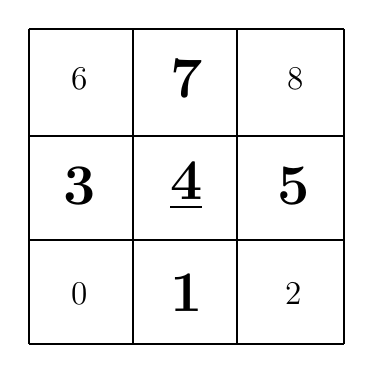
\begin{tikzpicture}[scale=4,thick]
\draw[-] (0,0)--(0,0.33);
\draw[-] (0,0.33)--(0,0.66);
\draw[-] (0,0.66)--(0,1);
\draw[-] (0.33,0)--(0.33,0.33);
\draw[-] (0.33,0.33)--(0.33,0.66);
\draw[-] (0.33,0.66)--(0.33,1);
\draw[-] (0.66,0)--(0.66,0.33);
\draw[-] (0.66,0.33)--(0.66,0.66);
\draw[-] (0.66,0.66)--(0.66,1);
\draw[-] (1,0)--(1,0.33);
\draw[-] (1,0.33)--(1,0.66);
\draw[-] (1,0.66)--(1,1);

\draw[-] (0,0)--(0.33,0);
\draw[-] (0.33,0)--(0.66,0);
\draw[-] (0.66,0)--(1,0);
\draw[-] (0,0.33)--(0.33,0.33);
\draw[-] (0.33,0.33)--(0.66,0.33);
\draw[-] (0.66,0.33)--(1,0.33);
\draw[-] (0,0.66)--(0.33,0.66);
\draw[-] (0.33,0.66)--(0.66,0.66);
\draw[-] (0.66,0.66)--(1,0.66);
\draw[-] (0,1)--(0.33,1);
\draw[-] (0.33,1)--(0.66,1);
\draw[-] (0.66,1)--(1,1);

\large
\draw (0.16,0.16) node {0};
\huge
\draw (0.5,0.16) node {\textbf{1}};
\large
\draw (0.84,0.16) node {2};
\huge
\draw (0.16,0.5) node {\textbf{3}};
\draw (0.5,0.5) node {\underline{\textbf{4}}};
\draw (0.84,0.5) node {\textbf{5}};
\large
\draw (0.16,0.84) node {6};
\huge
\draw (0.5,0.84) node {\textbf{7}};
\large
\draw (0.846,0.84) node {8};
\end{tikzpicture}
\caption[2-d neighbor map]{2-d neighbor enumeration. The current cell (in the
center) is underlined.}
\label{fig:neighbor_enumeration_2d}
\end{center}
\end{figure}

\begin{figure}[htp]
\begin{center}
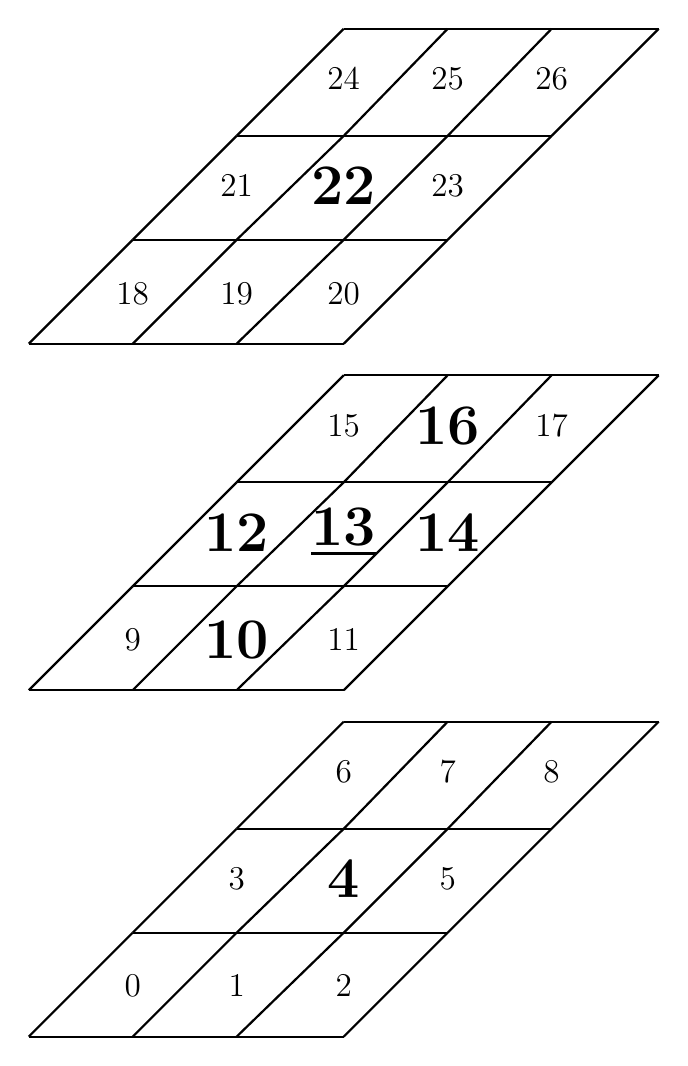
\begin{tikzpicture}[scale=4,thick]
%%%%%%%%%%%%%%%%%%%%%%%%%%%%%%%%
%% iz=0 layer
%%%%%%%%%%%%%%%%%%%%%%%%%%%%%%%%
\draw[-] (0,0)   --(0.33,0.33);
\draw[-] (0.33,0)--(0.66,0.33);
\draw[-] (0.66,0)--(1,0.33);
\draw[-] (1,0)   --(1.33,0.33);

\draw[-] (0.33,0.33)--(0.66,0.66);
\draw[-] (0.66,0.33)--(1,0.66);
\draw[-] (1,0.33)--(1.33,0.66);
\draw[-] (1.33,0.33)--(1.66,0.66);

\draw[-] (0.66,0.66)--(1,1);
\draw[-] (1.33,0.66)--(1.66,1);
\draw[-] (1,0.66)--(1.33,1);
\draw[-] (1.66,0.66)--(2,1);
%
\draw[-] (0,0)--(0.33,0);
\draw[-] (0.33,0)--(0.66,0);
\draw[-] (0.66,0)--(1,0);

\draw[-] (0.33,0.33)--(0.66,0.33);
\draw[-] (0.66,0.33)--(1,0.33);
\draw[-] (1,0.33)--(1.33,0.33);

\draw[-] (0.66,0.66)--(1,0.66);
\draw[-] (1,0.66)--(1.33,0.66);
\draw[-] (1.33,0.66)--(1.66,0.66);

\draw[-] (1,1)--(1.33,1);
\draw[-] (1.33,1)--(1.66,1);
\draw[-] (1.66,1)--(2,1);

\large
\draw (0.33,0.16) node {0};
\draw (0.66,0.16) node {1};
\draw (1,0.16) node {2};
\draw (0.66,0.5) node {3};
\huge
\draw (1,0.5) node {\textbf{4}};
\large
\draw (1.33,0.5) node {5};
\draw (1,0.84) node {6};
\draw (1.33,0.84) node {7};
\draw (1.66,0.84) node {8};
%
% 
%%%%%%%%%%%%%%%%%%%%%%%%%%%%%%%%
%% iz=1 layer
%%%%%%%%%%%%%%%%%%%%%%%%%%%%%%%%
\draw[-] (0,0+1.10)   --(0.33,0.33+1.10);
\draw[-] (0.33,0+1.10)--(0.66,0.33+1.10);
\draw[-] (0.66,0+1.10)--(1,0.33+1.10);
\draw[-] (1,0+1.10)   --(1.33,0.33+1.10);

\draw[-] (0.33,0.33+1.10)--(0.66,0.66+1.10);
\draw[-] (0.66,0.33+1.10)--(1,0.66+1.10);
\draw[-] (1,0.33+1.10)--(1.33,0.66+1.10);
\draw[-] (1.33,0.33+1.10)--(1.66,0.66+1.10);

\draw[-] (0.66,0.66+1.10)--(1,1+1.10);
\draw[-] (1.33,0.66+1.10)--(1.66,1+1.10);
\draw[-] (1,0.66+1.10)--(1.33,1+1.10);
\draw[-] (1.66,0.66+1.10)--(2,1+1.10);
%
\draw[-] (0,0+1.10)--(0.33,0+1.10);
\draw[-] (0.33,0+1.10)--(0.66,0+1.10);
\draw[-] (0.66,0+1.10)--(1,0+1.10);

\draw[-] (0.33,0.33+1.10)--(0.66,0.33+1.10);
\draw[-] (0.66,0.33+1.10)--(1,0.33+1.10);
\draw[-] (1,0.33+1.10)--(1.33,0.33+1.10);

\draw[-] (0.66,0.66+1.10)--(1,0.66+1.10);
\draw[-] (1,0.66+1.10)--(1.33,0.66+1.10);
\draw[-] (1.33,0.66+1.10)--(1.66,0.66+1.10);

\draw[-] (1,1+1.10)--(1.33,1+1.10);
\draw[-] (1.33,1+1.10)--(1.66,1+1.10);
\draw[-] (1.66,1+1.10)--(2,1+1.10);

\large
\draw (0.33,0.16+1.10) node {9};
\huge
\draw (0.66,0.16+1.10) node {\textbf{10}};
\large
\draw (1,0.16+1.10) node {11};
\huge
\draw (0.66,0.5+1.10) node {\textbf{12}};
\draw (1,0.5+1.10) node {\underline{\textbf{13}}};
\draw (1.33,0.5+1.10) node {\textbf{14}};
\large
\draw (1,0.84+1.10) node {15};
\huge
\draw (1.33,0.84+1.10) node {\textbf{16}};
\large
\draw (1.66,0.84+1.10) node {17};
%%%%%%%%%%%%%%%%%%%%%%%%%%%%%%%%
%% iz=2 layer
%%%%%%%%%%%%%%%%%%%%%%%%%%%%%%%%
\draw[-] (0,0+2.20)   --(0.33,0.33+2.20);
\draw[-] (0.33,0+2.20)--(0.66,0.33+2.20);
\draw[-] (0.66,0+2.20)--(1,0.33+2.20);
\draw[-] (1,0+2.20)   --(1.33,0.33+2.20);

\draw[-] (0.33,0.33+2.20)--(0.66,0.66+2.20);
\draw[-] (0.66,0.33+2.20)--(1,0.66+2.20);
\draw[-] (1,0.33+2.20)--(1.33,0.66+2.20);
\draw[-] (1.33,0.33+2.20)--(1.66,0.66+2.20);

\draw[-] (0.66,0.66+2.20)--(1,1+2.20);
\draw[-] (1.33,0.66+2.20)--(1.66,1+2.20);
\draw[-] (1,0.66+2.20)--(1.33,1+2.20);
\draw[-] (1.66,0.66+2.20)--(2,1+2.20);
%
\draw[-] (0,0+2.20)--(0.33,0+2.20);
\draw[-] (0.33,0+2.20)--(0.66,0+2.20);
\draw[-] (0.66,0+2.20)--(1,0+2.20);

\draw[-] (0.33,0.33+2.20)--(0.66,0.33+2.20);
\draw[-] (0.66,0.33+2.20)--(1,0.33+2.20);
\draw[-] (1,0.33+2.20)--(1.33,0.33+2.20);

\draw[-] (0.66,0.66+2.20)--(1,0.66+2.20);
\draw[-] (1,0.66+2.20)--(1.33,0.66+2.20);
\draw[-] (1.33,0.66+2.20)--(1.66,0.66+2.20);

\draw[-] (1,1+2.20)--(1.33,1+2.20);
\draw[-] (1.33,1+2.20)--(1.66,1+2.20);
\draw[-] (1.66,1+2.20)--(2,1+2.20);

\large
\draw (0.33,0.16+2.20) node {18};
\draw (0.66,0.16+2.20) node {19};
\draw (1,0.16+2.20) node {20};
\draw (0.66,0.5+2.20) node {21};
\huge
\draw (1,0.5+2.20) node {\textbf{22}};
\large
\draw (1.33,0.5+2.20) node {23};
\draw (1,0.84+2.20) node {24};
\draw (1.33,0.84+2.20) node {25};
\draw (1.66,0.84+2.20) node {26};
\end{tikzpicture}
\caption[2-d neighbor map]{3-d neighbor enumeration. The current cell (in the
center) is underlined.}
\label{fig:neighbor_enumeration_3d}
\end{center}
\end{figure}

%%%%%%%%%%%%%%%%%%%%%%%%%%%%%%%%%%%%%%%%%%%%%%%%%%%%%%%%%%%
\section{Grid traversal}
%%%%%%%%%%%%%%%%%%%%%%%%%%%%%%%%%%%%%%%%%%%%%%%%%%%%%%%%%%%
Peano does not store all cells as objects in a large data structure but 
does only initialize 1+$2^d$ cell objects.
One object is necessary for the storage of the parent cell
(coarse grid cell), the remaining are used to store its children
(fineGridCell).

During the traversal, parameters like position and dimensions of the 
a parent cell and its children are computed/loaded into this data structure. 
This idea is named the \textit{flyweight pattern}; cf.~ \cite{gangoffour}.   
Note that the root cell and its vertices are on level one (1) of the grid,
its children belong to level two (2).

Note further that after refinement, the final ``grid'' is defined by the fine
grid vertices/cells not by the coarse grid vertices/cells in our implementation!


Once:
\begin{enumerate}
  \item InitCells: beginIteration(): allocate CellDescription and data heap data
  memory
  \item InitCellData: initalize Update and Solution
\end{enumerate}

Every traversal:
\begin{enumerate}
  \item UpdateCellData: 
  \item ComputeCellData:
  \item ExtrapolateFaceData:
  \item ExchangeFaceData: 
\end{enumerate}

\section{Next steps}
\begin{enumerate}
  \item AMR: Introduce parent CellDescriptions that do not necessarily hold data
  but refer to the CellDescription indices of their child processes
  \item Plotting for high-order methods
  \item User templates for plotting so that we do not have to generate them
  everytime.
\end{enumerate}

\chapter{Examples}
\section{Step-12}
We consider a problem setting similar to the one in
\href{http://www.dealii.org/developer/doxygen/deal.II/step_12.html}{The
step-12 tutorial program}:
Given is a domain $\Omega=(0,1)^2$; inside the domain and on its boundary acts
a circular counterclockwise flow field
\begin{align}
\vec{b} &= \frac{1}{\sqrt{x^2+y^2}}(-y,x)
\end{align}
We have the following inflow boundary conditions:
\begin{align}
\inflow(t) &=
\begin{cases}
1 & \textup{for } \vec{x}\in [0,0.5]\times\{0\} \\
0 & \textup{otherwise}
\end{cases}
\end{align}

Note that according to the definition of the flow field, we only have one inflow
boundary, the boundary at $y=0$.
% bibliography
\bibliographystyle{siam}
\bibliography{bibliography}{}

\end{document}